%% LaTeX Beamer presentation template 
%% für den Lehrstuhl Paralleles Rechnen
%% am Wilhelm-Schickard-Institut der Universität Tübingen

%% Versions:
%% 0.9: 081014, Philip Effinger
%% 0.91: 110214, Philip Effinger: Anpassung an das neue CD der Universität 

%% Eine sehr gute Einführung in das Beamer-Package bietet der BEAMER_GUIDE
%% zuletzt gesehen unter: 
%% faq.ktug.or.kr/wiki/uploads/beamer_guide.pdf

\documentclass[compress]{beamer}

\mode<presentation>
{
% Das Theme für Beamer:
\usetheme{Darmstadt}
%möglich ist auch {Frankfurt}

% Farbe passend zum Unilogo
\usecolortheme[rgb={0.65,0.18,0.215}]{structure}

\usefonttheme{professionalfonts}

%Anzeigen der Seitenzahlen
\setbeamertemplate{footline}[frame number]


% Aufzählungspunkte sollen verdeckt sein, wenn sie noch nicht aktuell sind
\setbeamercovered{invisible}
% falls erwünscht, so kann auch {transparent} gewählt werden

% Navigationssymbole werden ausgeblendet
\setbeamertemplate{navigation symbols}{}}

% Wenn die aktuelle Folien rechts unten erscheinen soll
%\setbeamertemplate{footline}[frame number]

\usepackage[ngerman]{babel}

% Deutsche TeX-Eigenheiten
\usepackage{ngerman}

%deutsche Bibtex interpretation
\usepackage{bibgerm}

% Pakete für angenehmes Encoding
\usepackage[utf8x]{inputenc}
% \usepackage[T1]{fontenc}
%\usepackage{inputenc}


%% Für Bild in Tabelle
\newcommand\tabbild[2][]{%
	\raisebox{0pt}[\dimexpr\totalheight+\dp\strutbox\relax][\dp\strutbox]{%
		\includegraphics[#1]{#2}%
	}%
}

\usepackage{array}
\newcolumntype{C}[1]{>{\centering\arraybackslash}m{#1}}

% Tabelle-Zelle vertikal verbinden
\usepackage{multirow}

% für die Benutzung von Farben und Bildern
\usepackage{pgf}

% Verwendete Schriftarten
 \usepackage{mathptmx}
 \usepackage[scaled=.90]{helvet}
 \usepackage {amsmath, amssymb}


% %Für die Graphen
\usepackage {amsmath, amssymb}
\usepackage {graphicx}
\usepackage {tikz}
\usetikzlibrary {positioning, shadows, arrows, automata}

% Falls folgende Schriftart beim Kompilieren nicht gefunden wird, die Zeile
% bitte auskommentieren
\usepackage{avant}

% Die Daten für die pdf-Datei
\hypersetup{
	pdftitle={Masterarbeit:\\Untersuchung zur Machbarkeit von simultanem Eye-Tracking bei Menschengruppen mit Anwendungen im Klassenzimmer}
	pdfsubject={Masterarbeit Informatik}
	pdfauthor={Falko Benezan}
	pdfkeywords={Schluesselworte}
	pdfpagemode={FullScreen}
}

% Titelseite
\title{Untersuchung zur Machbarkeit von simultanem Eye-Tracking bei Menschengruppen mit Anwendungen im Klassenzimmer}
%\titlegraphic{
\includegraphics[height=1.5cm]{unilogo-rot} \qquad
%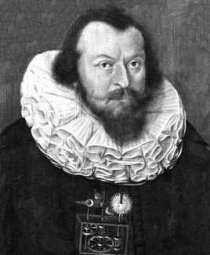
\includegraphics[height=2cm]{Wilhelm_Schickard}}

\author{Falko Benezan} 

\institute[Universität Tübingen]
{
Mathematisch-Naturwissenschaftliche Fakult"at \\
Wilhelm-Schickard-Institut f"ur Informatik
}

\date{\today}

% Wenn das Universitätslogo auf jeder Seite rechts unten klein erscheinen soll
 %\pgfdeclareimage[height=0.5cm]{university-logo}{./images/unilogo}
 %\logo{\pgfuseimage{university-logo}}


% Die Einblendung des Inhaltsverzeichnis am Beginn einer Sektion ist eigentlich
% nicht nötig
% \AtBeginSubsection[]
% {
% \begin{frame}<beamer>
% \frametitle{Outline}
% \tableofcontents[currentsection,currentsubsection]
% \end{frame}
% }

% Aktiviere schrittweises Einblenden bei Aufzählungen

\beamerdefaultoverlayspecification{<+->}
 
\begin{document}
 
\begin{frame}
\begin{center}
	\begin{huge}
		Masterarbeit Informatik
	\end{huge}
\end{center}
\titlepage
\end{frame}

% Der Rest des Templates ist eine kurze Einführung in:
% - die verschiedenen Overlay-Möglichkeiten von Beamer
% - die Benutzung von (Unter-)Sektionen in Beamer
%\frame{\frametitle{Gliederung}}
%\frame{\frametitle{Gliederung} \tableofcontents[sections={4-8}]}
\section{Intention}
\subsection{Klassenzimmer als Eye-Tracking Umgebung}
\begin{frame}
\begin{center}
	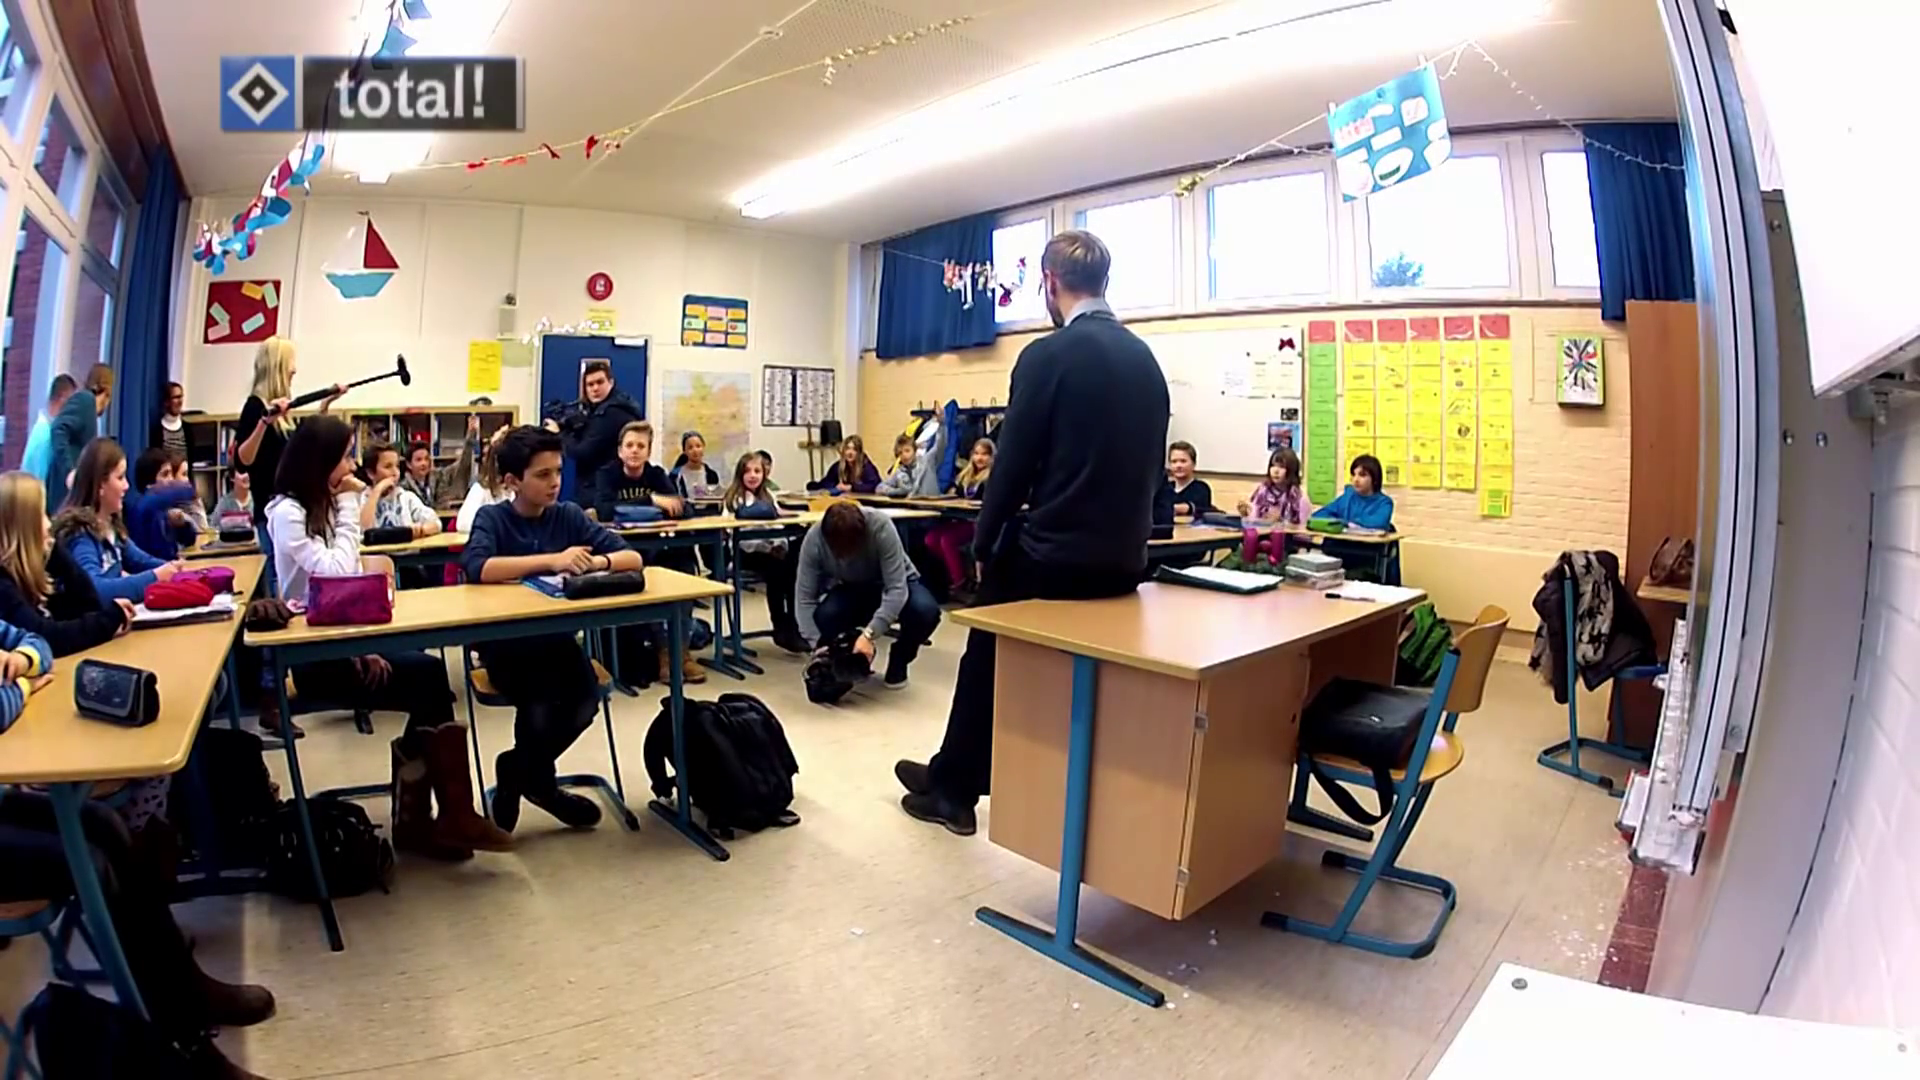
\includegraphics[width=0.55\linewidth]{images/Schulklasse}
\end{center}
\begin{itemize}
	\item<1-> Blickrichtung und Gesichtsorientierung der Schüler sollen so exakt wie möglich erfasst werden.
	\item<1-> Das Verfahren muss gleichzeitig auf $2,5 - 8m$ bei einer Breite von $6m$ funktionieren.\\
	Klassenzimmer: $54-66m^2$ für max. $31$ Schüler
	\item<1-> Der Unterricht soll durch die Aufnahme möglichst wenig gestört werden
	\item<1-> Die Aufnahme der Schulklasse erfolgt innerhalb eines Gebäudes
\end{itemize}
\end{frame}
\subsection{Umsetzung Graph}
\begin{frame}
\begin{center}
\begin{footnotesize}
\begin{tikzpicture}
	\node[circle,draw,align=center] (C) at(0,0) {Kamera};
	\node[draw,align=center] (F) at(0,-2)  {Gesichtserkennung};
	\node[draw,align=center] (S) at(0,-3.1)  {Skalierung};
	\node[draw,align=center] (G) at(6,-4.2)  {Graukonvertierung};
	\node[draw,align=center] (A) at(0,-4.2)  {Gesichtsanalyse};
	\node[draw,align=center] (E) at(6,-5.3)  {Augenanalyse};
	
	\node (outA) at(0,-7.3)  {};
	\node (outB) at(6,-7.3)  {};
	
	\draw[->] (E)to node[right,align=center]{Blickrichtung}(outB);
	\draw[->] (A)to[out=-45,in=90] node[right]{}(outB);
	
	\draw[->] (C)to node[right]{Frame}(F);
	\draw[->] (F)to node[right]{Bildausschnitt}(S);
	\draw[->] (S)to node[right]{Eingabebild}(A);
	\draw[->] (A)to node[left,align=center]{Gesichts-\\orientierung}(outA);
	
	\draw[->] (A)to node[below]{Augenbereich}(G);
	\draw[->] (C)to[out=-45,in=90] node[left]{}(G);
	\draw[->] (G)to node[right]{Eingabebild}(E);
\end{tikzpicture}
\end{footnotesize}
\end{center}
\end{frame} % Anstelle von Gliederung
\section{Gesichtserkennung}
\subsection{Detektion mit MTCNN}
\begin{frame}
Verarbeitung von Multi-task Cascaded Convolutional Networks (MTCNN)
\begin{columns}
	\begin{column}{0.59\linewidth}<1->
\begin{itemize}
	\item<1-> Bildpyramide auf der Eingabe
	\item<1-> Die 3 Stufen:
	\begin{enumerate}
		\item<1-> Proposal Network (P-Net):
		\item<1-> Refine Network (R-Net):
		\item<1-> Output Network (O-Net):
	\end{enumerate}
	\item<1-> Non-maximum suppression (NMS)
	\item<1-> Zuverlässige Detektion und Erkennen von $20\times 20$ Pixel große Gesichter möglich.
\end{itemize}
	\end{column}
	\begin{column}{0.41\linewidth}<1->
		\centering
		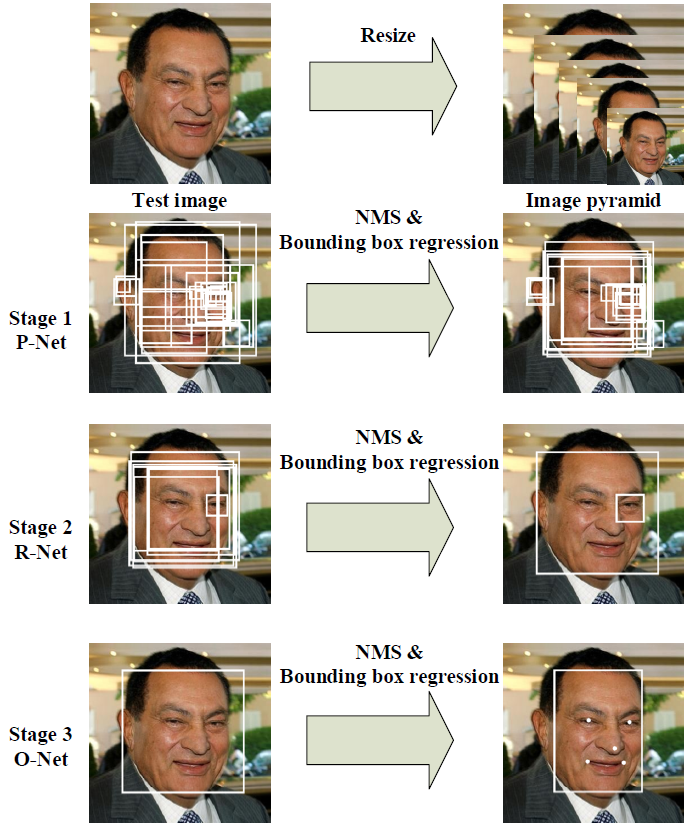
\includegraphics[width=\linewidth]{images/MTCNN_Step}
	\end{column}
\end{columns}
\end{frame}
\subsection{Verwendbarkeit im Versuch}
\begin{frame}
\begin{center}
	\begin{tabular}{|c|c|c|c|c|c|c|c|c|c|c|}
		\hline
		\tabbild[width=0.05\linewidth]{img_MTCNN/Img1-4_pupil1}&
		\tabbild[width=0.05\linewidth]{img_MTCNN/Img2-4_pupil1}&
		\tabbild[width=0.05\linewidth]{img_MTCNN/Img3-4_pupil1}&
		\tabbild[width=0.05\linewidth]{img_MTCNN/Img4-4_pupil1}&
		\tabbild[width=0.05\linewidth]{img_MTCNN/Img5-4_pupil1}&
		\tabbild[width=0.05\linewidth]{img_MTCNN/Img6-4_pupil1}&
		\tabbild[width=0.05\linewidth]{img_MTCNN/Img7-4_pupil1}&
		\tabbild[width=0.05\linewidth]{img_MTCNN/Img8-4_pupil1}&
		\tabbild[width=0.05\linewidth]{img_MTCNN/Img9-4_pupil1}&
		\tabbild[width=0.05\linewidth]{img_MTCNN/Img10-4_pupil1}&
		\tabbild[width=0.05\linewidth]{img_MTCNN/Img11-4_pupil1}\\
		{\fontsize{5}{7}$170\times235$}&
		{\fontsize{5}{7}$86\times118$}&
		{\fontsize{5}{7}$62\times87$}&
		{\fontsize{5}{7}$48\times65$}&
		{\fontsize{5}{7}$38\times54$}&
		{\fontsize{5}{7}$32\times44$}&
		{\fontsize{5}{7}$27\times39$}&
		{\fontsize{5}{7}$23\times31$}&
		{\fontsize{5}{7}$20\times26$}&
		{\fontsize{5}{7}$18\times24$}&
		{\fontsize{5}{7}$16\times21$}\\\hline
		$1m$& $2m$& $3m$& $4m$& $5m$& $6m$& $7m$& $8m$& $9m$& $10m$& $11m$\\\hline
	\end{tabular}
	Aufnahmen mit der Actioncam $(2688\times 1520, 170^\circ)$
\end{center}
\begin{itemize}
\item<1-> Detektion von Gesichtern bis zu $11m$ möglich
\item<1-> Ungenaue Landmarks für Augen, Nase und Mundwinkel
\end{itemize}
\end{frame}

\section{Skalierung}
\subsection{Skalieren von Bildern}
Da die Berechnungen meist auf recht kleinen Bildausschnitten ausgeführt werden muss, müssen diese für die weiteren Rechenschritte Hochskaliert werden.\\
Dabei ist es wichtig, dass die Gesichtsmerkmale möglichst gut rekonstruiert werden damit die entsprechenden Landmarks gefunden und bestimmt werden können.
\subsubsection{Nearest-Neighbor}
Verwende gleicher Farbwert wie das Nächstgelegene Pixel. Dadurch werden nur die ehemaligen Pixel größer und das Gesicht wirkt sehr Kantig.\\
To Do! - Bsp Bilder
\subsubsection{Linear}
Dabei wird zwischen den umliegenden nächst gelegenen Pixel Interpoliert, wodurch weitere Farbwerte entstehen und das Ergebnis gleichmäßiger aber unscharf wirkt.
To Do! - Bsp Bilder
\subsubsection{Bicubic}
Um den Farbwert zu ermitteln, werden die umliegenden $4\times 4$ Pixelwerte betrachtet um den Farbverlauf als eine Funktion 3. Grades zu bestimmen. Somit werden feinere Details besser dargestellt als beim Linearen verfahren, allerdings kann es durch den bestimmten Verlauf auch zum Überschwingen kommen, wodurch Fehlfarben entstehen können.\\
To Do! - Bsp Bilder
%%https://en.wikipedia.org/wiki/Bicubic_interpolation
\subsubsection{Lanczos}
Dieser Filter besteht aus einer Sinc-Funktion über einen Bereich, um so eine Bewertung der Benachbarten Pixelwerte zu erhalten. Somit kann ergibt sich der Neue Farbwert aus den bewerteten umliegenden Pixeln.\\
To Do! - Bsp Bilder
%%To Do! - Bsp Bilder

%% http://docs.opencv.org/2.4/modules/imgproc/doc/geometric_transformations.html#resize
\section{Gesichtsanalyse}
\subsection{OpenFace}
\begin{frame}
Einsatz eines Conditional Local Neural Fields (CLNF) für die Landmark-Detektion
\begin{itemize}
	\item<1-> 68 Gesichts-Landmarks
	\item<1-> 28 Augen-Landmarks
	\item<1-> Zuverlässig ab 100 Pixel große Gesichter
\end{itemize}
Zuverlässigkeit der Bestimmung von Position und Orientierung
\begin{itemize}
	\item<1-> Rotation auf BIWI: $6^\circ$
	\item<1-> Position auf BIWI: $2,5cm$ bei $95cm$
\end{itemize}
\end{frame}
\subsection{Auswirkung auf die Berechnung}
\begin{frame}
\begin{center}
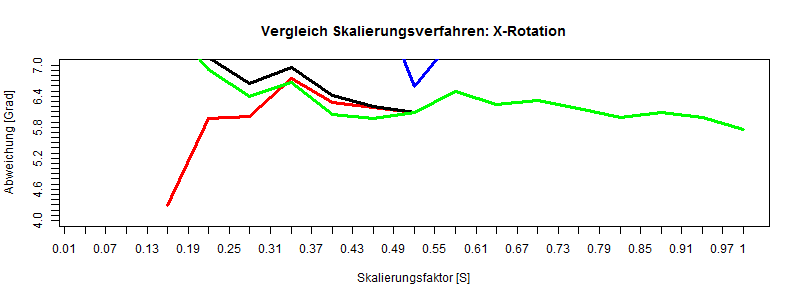
\includegraphics[width=0.49\linewidth]{img_Skal/Skal_Diff_RX}
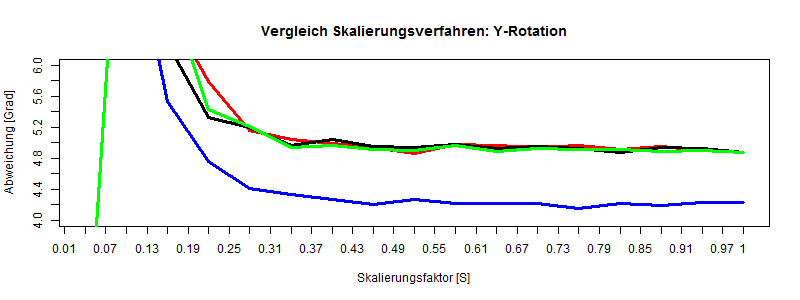
\includegraphics[width=0.49\linewidth]{img_Skal/Skal_Diff_RY}\\
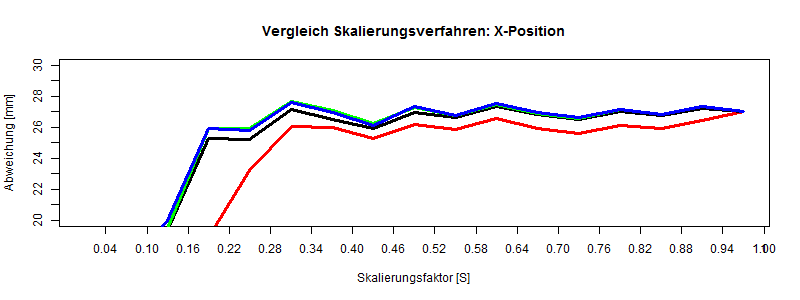
\includegraphics[width=0.49\linewidth]{img_Skal/Skal_Diff_TX}
\includegraphics[width=0.49\linewidth]{img_Skal/Skal_Diff_Tz}\\
\footnotesize{Bicubic (blau), Lanczos (grün), Linear (schwarz), N.-Neighbor (rot)}
\end{center}
\end{frame}

\section{Graukonvertierung}
\subsection{Umsetzung Graph}
\begin{frame}
\begin{center}
\begin{footnotesize}
\begin{tikzpicture}
	\node[circle,draw,align=center] (C) at(0,0) {Kamera};
	\node[draw,align=center] (F) at(0,-2)  {Gesichtserkennung};
	\node[draw,align=center] (S) at(0,-3.1)  {Skalierung};
	\node[draw,align=center] (G) at(6,-4.2)  {Graukonvertierung};
	\node[draw,align=center] (A) at(0,-4.2)  {Gesichtsanalyse};
	\node[draw,align=center] (E) at(6,-5.3)  {Augenanalyse};
	
	\node (outA) at(0,-7.3)  {};
	\node (outB) at(6,-7.3)  {};
	
	\draw[->] (E)to node[right,align=center]{Blickrichtung}(outB);
	\draw[->] (A)to[out=-45,in=90] node[right]{}(outB);
	
	\draw[->] (C)to node[right]{Frame}(F);
	\draw[->] (F)to node[right]{Bildausschnitt}(S);
	\draw[->] (S)to node[right]{Eingabebild}(A);
	\draw[->] (A)to node[left,align=center]{Gesichts-\\orientierung}(outA);
	
	\draw[->] (A)to node[below]{Augenbereich}(G);
	\draw[->] (C)to[out=-45,in=90] node[left]{}(G);
	\draw[->] (G)to node[right]{Eingabebild}(E);
\end{tikzpicture}
\end{footnotesize}
\end{center}
\end{frame} % Anstelle von Gliederung
\subsection{Intention}
\begin{frame}
Für die Bestimmung der Blickrichtung hat die Augenregion eine besondere Bedeutung.
\begin{itemize}
	\item<1-> OpenFace verwendet Landmarks für das Augenlid, Iris und Pupille
	\item<1-> Bestimmung der Blickrichtung aus den Landmarks
	\item<1-> ElSe zur Bestimmung der Pupille
\end{itemize}
Verfahre muss stabil bei sehr keinen Bildern arbeiten.
\end{frame}
\begin{frame}
ElSe erwartet ein hochauflösendes Graubild des Auges mit hohem Kontrast zwischen Pupille und Iris.
\begin{figure}
	\centering
	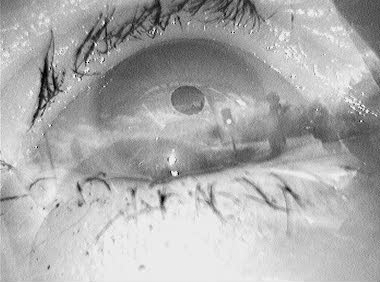
\includegraphics[height=0.3\textheight]{images/Eye_Gray}
	
\includegraphics[height=0.3\textheight]{images/Auge_4}
	\label{fig:eyegray}
\end{figure}
Eingabe ist ein niedrig aufgelöstes Farbbild.
\end{frame}
\subsection{Verfahren}
\begin{frame}
\begin{center}
\begin{columns}
	\begin{column}{\linewidth}<1->
		\begin{tabular}{|C{4.2cm}|C{2.03cm}|C{3.5cm}|}
		\hline
		Eingabebid&\tabbild[height=0.1\textheight]{images/Auge}&{\tiny $G_{new} = \dfrac{(G-G_{min})\cdot V_{max}}{G_{max}-G_{min}}$}\\\hline
		Gleam-Verfahren	&\tabbild[height=0.1\textheight]{images/Auge_2Gray}&{\tiny $\dfrac{R^{\frac{1}{2,2}} + G^{\frac{1}{2,2}} + B^{\frac{1}{2,2}}}{3}$}\\\hline
		Gleam-New-Verfahren&\tabbild[height=0.1\textheight]{images/Auge_1Gray}&{\scriptsize $\dfrac{R^{r} + G^{g} + B^{b}}{3},~\frac{\log(V_{\max})}{\log(\{R,G,B\}_{\max})}$}\\\hline
		Luminance-Verfahren&\tabbild[height=0.1\textheight]{images/Auge_0Gray}&{\scriptsize $0,299 R + 0,587 G + 0,114 B$}\\\hline
		Min-Verfahren&\tabbild[height=0.1\textheight]{images/Auge_4Gray}& $\min(R,G,B)$\\\hline
		Max-Verfahren&\tabbild[height=0.1\textheight]{images/Auge_5Gray}& $\max(R,G,B)$\\\hline
		Quadrat-Verfahren&\tabbild[height=0.1\textheight]{images/Auge_3Gray}&{\scriptsize $\dfrac{R^2+G^2+B^2}{3}$}\\\hline
		\end{tabular}
	\end{column}
\end{columns}
\end{center}
\end{frame}
\section{Augenanalyse}
\subsection{ElSe im Test}
\begin{frame}
\begin{figure}
	\centering
	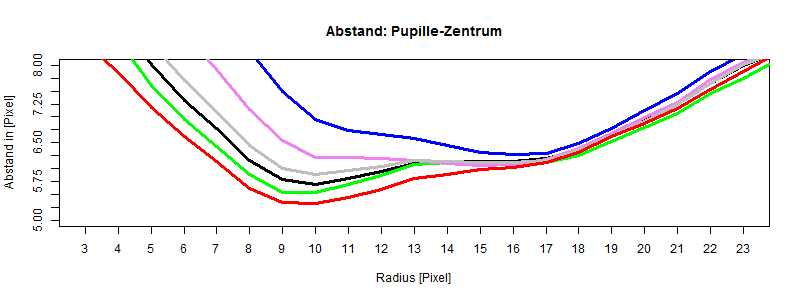
\includegraphics[width=\linewidth]{img_ElSe/Vergleich_A}
\end{figure}
Median-Abstand in Pixel des Zentrums der Pupille gegen die Veränderung des Radius des Filters.\\
Verfahren: Gleam (rot), Luminance (schwarz), Max (grün), Min (violett), New-Gleam (grau), Quadrat (blau)
\end{frame}
\begin{frame}
\begin{figure}
	\centering
	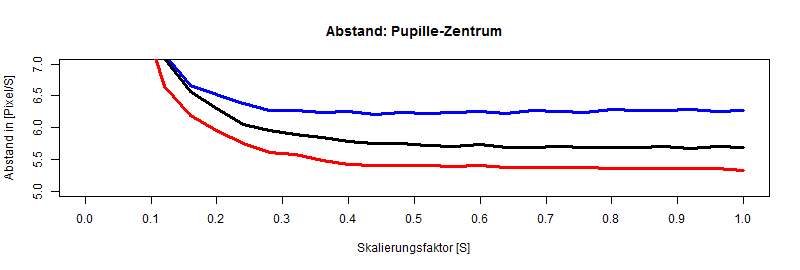
\includegraphics[width=0.8\linewidth]{img_ElSe/Vergleich_Scal_A}
	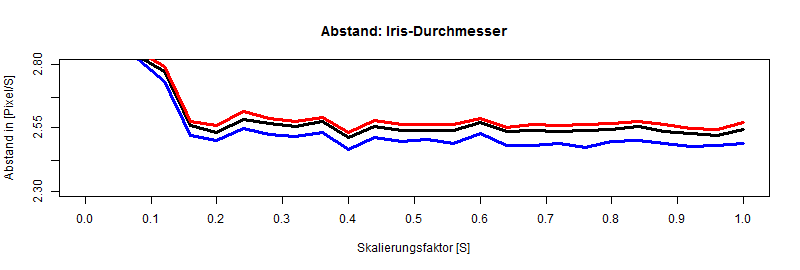
\includegraphics[width=0.8\linewidth]{img_ElSe/Vergleich_Scal_I}
\end{figure}
Abstand in Pixel zwischen der Berechnung und des Datensatzes bei verschiedenen Skalierungen.\\
Originaler durchschnittlicher Pupillendurchmesser 15 Pixel.\\
Gleam (rot), Luminance (schwarz),  Quadrat (blau)
\end{frame}
\subsection{OpenFace im Vergleich}
\begin{frame}
\begin{figure}
	\centering
	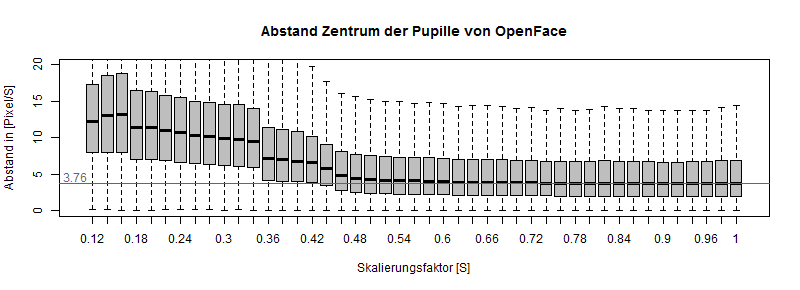
\includegraphics[width=0.8\linewidth]{img_ElSe/OpenFace_PC}
	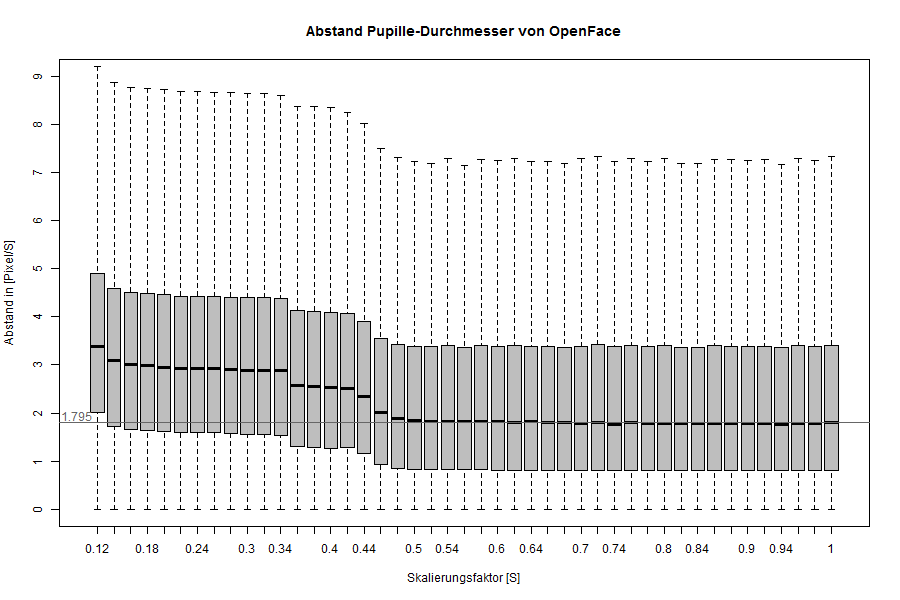
\includegraphics[width=0.8\linewidth]{img_ElSe/OpenFace_PW}
\end{figure}
Abstand in Pixel zwischen der Berechnung und des Datensatzes bei verschiedenen Skalierungen.\\
Originaler durchschnittlicher Irisdurchmesser 34 Pixel.\\
\end{frame}
\section{Versuche}
\subsection{Versuch 1}
\begin{frame}
Auswirkung der Position im Raum auf die Berechnung und horizontaler Arbeitsbereich
\begin{itemize}
	\item<1-> Probanden befinden sich auf einem $1\times 1m$ Raster.
	\item<1-> $2688\times 1520$ Farbkamera mit $170^\circ$ Weitwinkel-Linse und großer Schärfentiefe.
	\item<1-> Blick-Ziel sind weit verteilt an der Wand
\end{itemize}
\begin{figure}
	\centering
	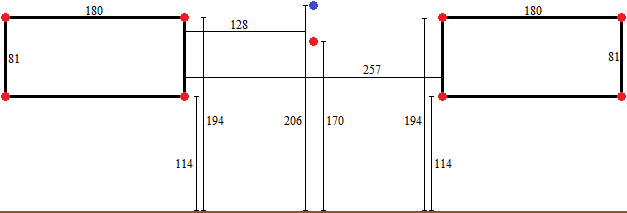
\includegraphics[width=0.7\linewidth]{images/Target}
\end{figure}
\end{frame}
\begin{frame}
\begin{center}
	\begin{tabular}{|c|c|c|c|c|c|}
	\hline 
	$+6m$ & &&&&\\
	\hline 
	$+5m$ &
	
\includegraphics[width=0.5cm]{img_Bereich/V1_img_Winkel_X_-2000_5000.png} &
	
\includegraphics[width=0.5cm]{img_Bereich/V1_img_Winkel_X_-1000_5000.png} &
	
\includegraphics[width=0.5cm]{img_Bereich/V1_img_Winkel_X_0_5000.png} &
	
\includegraphics[width=0.5cm]{img_Bereich/V1_img_Winkel_X_1000_5000.png} &
	
\includegraphics[width=0.5cm]{img_Bereich/V1_img_Winkel_X_2000_5000.png} \\ 
	\hline 
	$+4m$ &
	
\includegraphics[width=0.5cm]{img_Bereich/V1_img_Winkel_X_-2000_4000.png} &
	
\includegraphics[width=0.5cm]{img_Bereich/V1_img_Winkel_X_-1000_4000.png} &
	
\includegraphics[width=0.5cm]{img_Bereich/V1_img_Winkel_X_0_4000.png} &
	
\includegraphics[width=0.5cm]{img_Bereich/V1_img_Winkel_X_1000_4000.png} &
	
\includegraphics[width=0.5cm]{img_Bereich/V1_img_Winkel_X_2000_4000.png} \\ 
	\hline 
	$+3m$ &
	
\includegraphics[width=0.5cm]{img_Bereich/V1_img_Winkel_X_-2000_3000.png} &
	
\includegraphics[width=0.5cm]{img_Bereich/V1_img_Winkel_X_-1000_3000.png} &
	
\includegraphics[width=0.5cm]{img_Bereich/V1_img_Winkel_X_0_3000.png} &
	
\includegraphics[width=0.5cm]{img_Bereich/V1_img_Winkel_X_1000_3000.png} &
	
\includegraphics[width=0.5cm]{img_Bereich/V1_img_Winkel_X_2000_3000.png} \\ 
	\hline 
	$+2m$ &&
	
\includegraphics[width=0.5cm]{img_Bereich/V1_img_Winkel_X_-1000_2000.png} &
	
\includegraphics[width=0.5cm]{img_Bereich/V1_img_Winkel_X_0_2000.png} &
	
\includegraphics[width=0.5cm]{img_Bereich/V1_img_Winkel_X_1000_2000.png} & \\ 
	\hline 
	$+1m$ & &
	
\includegraphics[width=0.5cm]{img_Bereich/V1_img_Winkel_X_-1000_1000.png} &
	
\includegraphics[width=0.5cm]{img_Bereich/V1_img_Winkel_X_0_1000.png} &
	
\includegraphics[width=0.5cm]{img_Bereich/V1_img_Winkel_X_1000_1000.png} & \\ 
	\hline 
	& $-2m$ & $-1m$ &0& $+1m$ & $+2m$ \\ 
	\hline 
\end{tabular}
	\begin{tabular}{|c|c|c|c|c|c|c|c|}
	\hline
	$+6$ &
	
\includegraphics[width=0.045\linewidth]{img_Bereich/V1_vid_Winkel_X_-3000_5000.png}&
	
\includegraphics[width=0.045\linewidth]{img_Bereich/V1_vid_Winkel_X_-2000_5000.png}&
	
\includegraphics[width=0.045\linewidth]{img_Bereich/V1_vid_Winkel_X_-1000_5000.png}&
	
\includegraphics[width=0.045\linewidth]{img_Bereich/V1_vid_Winkel_X_0_5000.png}&
	
\includegraphics[width=0.045\linewidth]{img_Bereich/V1_vid_Winkel_X_1000_5000.png}&
	
\includegraphics[width=0.045\linewidth]{img_Bereich/V1_vid_Winkel_X_2000_5000.png}&\\ 
	\hline 
	$+5$ &
	
\includegraphics[width=0.045\linewidth]{img_Bereich/V1_vid_Winkel_X_-3000_5000.png}&
	
\includegraphics[width=0.045\linewidth]{img_Bereich/V1_vid_Winkel_X_-2000_5000.png}&
	
\includegraphics[width=0.045\linewidth]{img_Bereich/V1_vid_Winkel_X_-1000_5000.png}&
	
\includegraphics[width=0.045\linewidth]{img_Bereich/V1_vid_Winkel_X_0_5000.png}&
	
\includegraphics[width=0.045\linewidth]{img_Bereich/V1_vid_Winkel_X_1000_5000.png}&
	
\includegraphics[width=0.045\linewidth]{img_Bereich/V1_vid_Winkel_X_2000_5000.png}&\\ 
	\hline 
	$+4$ &
	\includegraphics[width=0.045\linewidth]{img_Bereich/V1_vid_Winkel_X_-3000_4000.png}&
	\includegraphics[width=0.045\linewidth]{img_Bereich/V1_vid_Winkel_X_-2000_4000.png}&
	\includegraphics[width=0.045\linewidth]{img_Bereich/V1_vid_Winkel_X_-1000_4000.png}&
	\includegraphics[width=0.045\linewidth]{img_Bereich/V1_vid_Winkel_X_0_4000.png}&
	\includegraphics[width=0.045\linewidth]{img_Bereich/V1_vid_Winkel_X_1000_4000.png}&
	\includegraphics[width=0.045\linewidth]{img_Bereich/V1_vid_Winkel_X_2000_4000.png}&
	\includegraphics[width=0.045\linewidth]{img_Bereich/V1_vid_Winkel_X_3000_4000.png}\\ 
	\hline 
	$+3$ &
	\includegraphics[width=0.045\linewidth]{img_Bereich/V1_vid_Winkel_X_-3000_3000.png}&
	\includegraphics[width=0.045\linewidth]{img_Bereich/V1_vid_Winkel_X_-2000_3000.png}&
	\includegraphics[width=0.045\linewidth]{img_Bereich/V1_vid_Winkel_X_-1000_3000.png}&
	\includegraphics[width=0.045\linewidth]{img_Bereich/V1_vid_Winkel_X_0_3000.png}&
	\includegraphics[width=0.045\linewidth]{img_Bereich/V1_vid_Winkel_X_1000_3000.png}&
	\includegraphics[width=0.045\linewidth]{img_Bereich/V1_vid_Winkel_X_2000_3000.png}&
	\includegraphics[width=0.045\linewidth]{img_Bereich/V1_vid_Winkel_X_3000_3000.png}\\ 
	\hline 
	$+2$ & &
	\includegraphics[width=0.045\linewidth]{img_Bereich/V1_vid_Winkel_X_-2000_2000.png}&
	\includegraphics[width=0.045\linewidth]{img_Bereich/V1_vid_Winkel_X_-1000_2000.png}&
	\includegraphics[width=0.045\linewidth]{img_Bereich/V1_vid_Winkel_X_0_2000.png}&
	\includegraphics[width=0.045\linewidth]{img_Bereich/V1_vid_Winkel_X_1000_2000.png}&
	\includegraphics[width=0.045\linewidth]{img_Bereich/V1_vid_Winkel_X_2000_2000.png}& \\ 
	\hline 
	$+1$ & & &
	\includegraphics[width=0.045\linewidth]{img_Bereich/V1_vid_Winkel_X_-1000_1000.png}&
	\includegraphics[width=0.045\linewidth]{img_Bereich/V1_vid_Winkel_X_0_1000.png}&
	\includegraphics[width=0.045\linewidth]{img_Bereich/V1_vid_Winkel_X_1000_1000.png}& &\\ 
	\hline 
	& $-3$& $-2$ & $-1$ &0& $+1$ & $+2$ & $+3$ \\ 
	\hline 
\end{tabular}
\end{center}
\end{frame}
\begin{frame}
\begin{center}
\begin{tabular}{|c|c|c|c|c|c|c|c|}
	\hline
	$+11m$ & & & &
	\includegraphics[width=1cm]{img_Bereich/V1_vid_res_Winkel_X_0_11000.png}& & &\\ 
	\hline 
	$+10m$ & & &
	\includegraphics[width=1cm]{img_Bereich/V1_vid_res_Winkel_X_-1000_10000.png}&
	\includegraphics[width=1cm]{img_Bereich/V1_vid_res_Winkel_X_0_10000.png}&
	\includegraphics[width=1cm]{img_Bereich/V1_vid_res_Winkel_X_1000_10000.png}&
	\includegraphics[width=1cm]{img_Bereich/V1_vid_res_Winkel_X_2000_10000.png}&\\ 
	\hline 
	$+9m$ & & &
	\includegraphics[width=1cm]{img_Bereich/V1_vid_res_Winkel_X_-1000_9000.png}&
	\includegraphics[width=1cm]{img_Bereich/V1_vid_res_Winkel_X_0_9000.png}&
	\includegraphics[width=1cm]{img_Bereich/V1_vid_res_Winkel_X_1000_9000.png}&
	\includegraphics[width=1cm]{img_Bereich/V1_vid_res_Winkel_X_2000_9000.png}&\\ 
	\hline 
	$+8m$ & & &
	\includegraphics[width=1cm]{img_Bereich/V1_vid_res_Winkel_X_-1000_8000.png}&
	\includegraphics[width=1cm]{img_Bereich/V1_vid_res_Winkel_X_0_8000.png}&
	\includegraphics[width=1cm]{img_Bereich/V1_vid_res_Winkel_X_1000_8000.png}& & \\ 
	\hline 
	$+7m$ & & &
	\includegraphics[width=1cm]{img_Bereich/V1_vid_res_Winkel_X_-1000_7000.png}&
	\includegraphics[width=1cm]{img_Bereich/V1_vid_res_Winkel_X_0_7000.png}&
	\includegraphics[width=1cm]{img_Bereich/V1_vid_res_Winkel_X_1000_7000.png}& & \\ 
	\hline 
	$+6m$ & & &
	\includegraphics[width=1cm]{img_Bereich/V1_vid_res_Winkel_X_-1000_6000.png}&
	\includegraphics[width=1cm]{img_Bereich/V1_vid_res_Winkel_X_0_6000.png}&
	\includegraphics[width=1cm]{img_Bereich/V1_vid_res_Winkel_X_1000_6000.png}&
	\includegraphics[width=1cm]{img_Bereich/V1_vid_res_Winkel_X_2000_6000.png}&
	\includegraphics[width=1cm]{img_Bereich/V1_vid_res_Winkel_X_3000_6000.png}\\ 
	\hline 
	$+5m$ &
	\includegraphics[width=1cm]{img_Bereich/V1_vid_res_Winkel_X_-3000_5000.png}& &
	\includegraphics[width=1cm]{img_Bereich/V1_vid_res_Winkel_X_-1000_5000.png}&
	\includegraphics[width=1cm]{img_Bereich/V1_vid_res_Winkel_X_0_5000.png}&
	\includegraphics[width=1cm]{img_Bereich/V1_vid_res_Winkel_X_1000_5000.png}&
	\includegraphics[width=1cm]{img_Bereich/V1_vid_res_Winkel_X_2000_5000.png}&
	\includegraphics[width=1cm]{img_Bereich/V1_vid_res_Winkel_X_3000_5000.png}\\ 
	\hline 
	$+4m$ &
	\includegraphics[width=1cm]{img_Bereich/V1_vid_res_Winkel_X_-3000_4000.png}& &
	\includegraphics[width=1cm]{img_Bereich/V1_vid_res_Winkel_X_-1000_4000.png}&
	\includegraphics[width=1cm]{img_Bereich/V1_vid_res_Winkel_X_0_4000.png}&
	\includegraphics[width=1cm]{img_Bereich/V1_vid_res_Winkel_X_1000_4000.png}&
	\includegraphics[width=1cm]{img_Bereich/V1_vid_res_Winkel_X_2000_4000.png}&
	\includegraphics[width=1cm]{img_Bereich/V1_vid_res_Winkel_X_3000_4000.png}\\ 
	\hline 
	$+3m$ &
	\includegraphics[width=1cm]{img_Bereich/V1_vid_res_Winkel_X_-3000_3000.png}& &
	\includegraphics[width=1cm]{img_Bereich/V1_vid_res_Winkel_X_-1000_3000.png}&
	\includegraphics[width=1cm]{img_Bereich/V1_vid_res_Winkel_X_0_3000.png}&
	\includegraphics[width=1cm]{img_Bereich/V1_vid_res_Winkel_X_1000_3000.png}&
	\includegraphics[width=1cm]{img_Bereich/V1_vid_res_Winkel_X_2000_3000.png}&
	\includegraphics[width=1cm]{img_Bereich/V1_vid_res_Winkel_X_3000_3000.png}\\ 
	\hline 
	$+2m$ & & &
	\includegraphics[width=1cm]{img_Bereich/V1_vid_res_Winkel_X_-1000_2000.png}&
	\includegraphics[width=1cm]{img_Bereich/V1_vid_res_Winkel_X_0_2000.png}&
	\includegraphics[width=1cm]{img_Bereich/V1_vid_res_Winkel_X_1000_2000.png}&
	\includegraphics[width=1cm]{img_Bereich/V1_vid_res_Winkel_X_2000_2000.png}&\\ 
	\hline 
	$+1m$ & & &
	\includegraphics[width=1cm]{img_Bereich/V1_vid_res_Winkel_X_-1000_1000.png}&
	\includegraphics[width=1cm]{img_Bereich/V1_vid_res_Winkel_X_0_1000.png}&
	\includegraphics[width=1cm]{img_Bereich/V1_vid_res_Winkel_X_1000_1000.png}& &\\ 
	\hline 
	& $-3m$ & $-2m$ & $-1m$ &Kamera& $+1m$ & $+2m$ & $+3m$ \\ 
	\hline 
\end{tabular}
\end{center}
\end{frame}
\subsection{Versuch 2}
\begin{frame}
Verkürzter Versuch um den vertikalen Arbeitsbereich zu Untersuchen.
\begin{itemize}
	\item<1-> Der Proband befindet sich auf einer Linie $3m$ und $9m$ entfernt
	\item<1-> Blick-Ziel befinden sich zu meist $1m$ auf dem Boden vor den Linien.
	\item<1-> $2688\times 1520$ Farbkamera mit $170^\circ$ Weitwinkel-Linse und großer Schärfentiefe.
\end{itemize}
\end{frame}
\begin{frame}
\begin{center}
	\begin{tabular}{|c|c|c|c|c|c|c|c|c|}
	\hline 
	$+3m$ & &
	\includegraphics[width=0.5cm]{img_Bereich/V2_img_Winkel_Y_-2000_3000.png}&
	\includegraphics[width=0.5cm]{img_Bereich/V2_img_Winkel_Y_-1000_3000.png}&
	\includegraphics[width=0.5cm]{img_Bereich/V2_img_Winkel_Y_0_3000.png}&
	\includegraphics[width=0.5cm]{img_Bereich/V2_img_Winkel_Y_1000_3000.png}&
	\includegraphics[width=0.5cm]{img_Bereich/V2_img_Winkel_Y_2000_3000.png}&
	\includegraphics[width=0.5cm]{img_Bereich/V2_img_Winkel_Y_3000_3000.png}&\\ 
	\hline 
	& $-3m$ & $-2m$ & $-1m$ &Kamera& $+1m$ & $+2m$ & $+3m$ & $+4m$ \\ 
	\hline
	\hline 
	$+3m$ &
	\includegraphics[width=0.5cm]{img_Bereich/V2_vid_Winkel_Y_-3000_3000.png}&
	\includegraphics[width=0.5cm]{img_Bereich/V2_vid_Winkel_Y_-2000_3000.png}&
	\includegraphics[width=0.5cm]{img_Bereich/V2_vid_Winkel_Y_-1000_3000.png}&
	\includegraphics[width=0.5cm]{img_Bereich/V2_vid_Winkel_Y_0_3000.png}&
	\includegraphics[width=0.5cm]{img_Bereich/V2_vid_Winkel_Y_1000_3000.png}&
	\includegraphics[width=0.5cm]{img_Bereich/V2_vid_Winkel_Y_2000_3000.png}&
	\includegraphics[width=0.5cm]{img_Bereich/V2_vid_Winkel_Y_3000_3000.png}&
	\includegraphics[width=0.5cm]{img_Bereich/V2_vid_Winkel_Y_4000_3000.png}\\ 
	\hline 
	& $-3m$ & $-2m$ & $-1m$ &Kamera& $+1m$ & $+2m$ & $+3m$ & $+4m$ \\ 
	\hline 
\end{tabular}
	\begin{tabular}{|c|c|c|c|c|c|c|c|c|}
	\hline 
	$+9m$ &
	\includegraphics[width=0.5cm]{img_Bereich/V2_img_res_Winkel_Y_-3000_9000.png}&
	\includegraphics[width=0.5cm]{img_Bereich/V2_img_res_Winkel_Y_-2000_9000.png}&
	\includegraphics[width=0.5cm]{img_Bereich/V2_img_res_Winkel_Y_-1000_9000.png}&
	\includegraphics[width=0.5cm]{img_Bereich/V2_img_res_Winkel_Y_0_9000.png}&
	\includegraphics[width=0.5cm]{img_Bereich/V2_img_res_Winkel_Y_1000_9000.png}&
	\includegraphics[width=0.5cm]{img_Bereich/V2_img_res_Winkel_Y_2000_9000.png}&
	\includegraphics[width=0.5cm]{img_Bereich/V2_img_res_Winkel_Y_3000_9000.png}&
	\includegraphics[width=0.5cm]{img_Bereich/V2_img_res_Winkel_Y_4000_9000.png}\\ 
	\hline 
	$+3m$ & &
	\includegraphics[width=0.5cm]{img_Bereich/V2_img_res_Winkel_Y_-2000_3000.png}&
	\includegraphics[width=0.5cm]{img_Bereich/V2_img_res_Winkel_Y_-1000_3000.png}&
	\includegraphics[width=0.5cm]{img_Bereich/V2_img_res_Winkel_Y_0_3000.png}&
	\includegraphics[width=0.5cm]{img_Bereich/V2_img_res_Winkel_Y_1000_3000.png}&
	\includegraphics[width=0.5cm]{img_Bereich/V2_img_res_Winkel_Y_2000_3000.png}&
	\includegraphics[width=0.5cm]{img_Bereich/V2_img_res_Winkel_Y_3000_3000.png}&
	\includegraphics[width=0.5cm]{img_Bereich/V2_img_res_Winkel_Y_4000_3000.png}\\ 
	\hline 
	& $-3m$ & $-2m$ & $-1m$ &Kamera& $+1m$ & $+2m$ & $+3m$ & $+4m$ \\ 
	\hline
	\hline 
	$+9m$ &
	\includegraphics[width=0.5cm]{img_Bereich/V2_vid_res_Winkel_Y_-3000_9000.png}&
	\includegraphics[width=0.5cm]{img_Bereich/V2_vid_res_Winkel_Y_-2000_9000.png}&
	\includegraphics[width=0.5cm]{img_Bereich/V2_vid_res_Winkel_Y_-1000_9000.png}&
	\includegraphics[width=0.5cm]{img_Bereich/V2_vid_res_Winkel_Y_0_9000.png}&
	\includegraphics[width=0.5cm]{img_Bereich/V2_vid_res_Winkel_Y_1000_9000.png}&
	\includegraphics[width=0.5cm]{img_Bereich/V2_vid_res_Winkel_Y_2000_9000.png}&
	\includegraphics[width=0.5cm]{img_Bereich/V2_vid_res_Winkel_Y_3000_9000.png}&
	\includegraphics[width=0.5cm]{img_Bereich/V2_vid_res_Winkel_Y_4000_9000.png}\\ 
	\hline 
	$+3m$ &
	\includegraphics[width=0.5cm]{img_Bereich/V2_vid_res_Winkel_Y_-3000_3000.png}&
	\includegraphics[width=0.5cm]{img_Bereich/V2_vid_res_Winkel_Y_-2000_3000.png}&
	\includegraphics[width=0.5cm]{img_Bereich/V2_vid_res_Winkel_Y_-1000_3000.png}&
	\includegraphics[width=0.5cm]{img_Bereich/V2_vid_res_Winkel_Y_0_3000.png}&
	\includegraphics[width=0.5cm]{img_Bereich/V2_vid_res_Winkel_Y_1000_3000.png}&
	\includegraphics[width=0.5cm]{img_Bereich/V2_vid_res_Winkel_Y_2000_3000.png}&
	\includegraphics[width=0.5cm]{img_Bereich/V2_vid_res_Winkel_Y_3000_3000.png}&
	\includegraphics[width=0.5cm]{img_Bereich/V2_vid_res_Winkel_Y_4000_3000.png}\\ 
	\hline 
	& $-3m$ & $-2m$ & $-1m$ &Kamera& $+1m$ & $+2m$ & $+3m$ & $+4m$ \\ 
	\hline 
\end{tabular}{\tiny }
\end{center}
\end{frame}
\subsection{Versuch 3}
\begin{frame}
	Fotokamera mit $6000 \times 4000$ Farbbild\\
	\begin{tabular}{|c|c|c|c|c|c|c|c|}
\hline 
$+12m$&&&
\includegraphics[width=0.115\linewidth]{Auge1/A_Img12-3FalkoE.png} &
\includegraphics[width=0.115\linewidth]{Auge1/A_Img12-4FalkoE.png}  &
\includegraphics[width=0.115\linewidth]{Auge1/A_Img12-5FalkoE.png} && \\ 
&&&&
\includegraphics[width=0.115\linewidth]{Auge1/A_Img12-4ThomasE.png}  &
\includegraphics[width=0.115\linewidth]{Auge1/A_Img12-5ThomasE.png} && \\ \hline 
$+11m$&&&
\includegraphics[width=0.115\linewidth]{Auge1/A_Img11-3FalkoE.png} &
\includegraphics[width=0.115\linewidth]{Auge1/A_Img11-4FalkoE.png} &
\tabbild[width=0.115\linewidth]{Auge1/A_Img11-5FalkoE.png} &
&
\\
&&&
\includegraphics[width=0.115\linewidth]{Auge1/A_Img11-3ThomasE.png} &
\includegraphics[width=0.115\linewidth]{Auge1/A_Img11-4ThomasE.png} &
\includegraphics[width=0.115\linewidth]{Auge1/A_Img11-5ThomasE.png} &
&\\\hline 
$+10m$&
\includegraphics[width=0.115\linewidth]{Auge1/A_Img10-1FalkoE.png} &
\includegraphics[width=0.115\linewidth]{Auge1/A_Img10-2FalkoE.png} &
\includegraphics[width=0.115\linewidth]{Auge1/A_Img10-3FalkoE.png} &
\includegraphics[width=0.115\linewidth]{Auge1/A_Img10-4FalkoE.png} &
\tabbild[width=0.115\linewidth]{Auge1/A_Img10-5FalkoE.png} &
\includegraphics[width=0.115\linewidth]{Auge1/A_Img10-6FalkoE.png} &
\includegraphics[width=0.115\linewidth]{Auge1/A_Img10-7FalkoE.png} \\&
\includegraphics[width=0.115\linewidth]{Auge1/A_Img10-1ThomasE.png} &
\includegraphics[width=0.115\linewidth]{Auge1/A_Img10-2ThomasE.png} &
\includegraphics[width=0.115\linewidth]{Auge1/A_Img10-3ThomasE.png} &
\includegraphics[width=0.115\linewidth]{Auge1/A_Img10-4ThomasE.png} &
\includegraphics[width=0.115\linewidth]{Auge1/A_Img10-5ThomasE.png} &
\includegraphics[width=0.115\linewidth]{Auge1/A_Img10-6ThomasE.png} &
\includegraphics[width=0.115\linewidth]{Auge1/A_Img10-7ThomasE.png} \\\hline 
$+9m$&
\includegraphics[width=0.115\linewidth]{Auge1/A_Img9-1FalkoE.png} &
\includegraphics[width=0.115\linewidth]{Auge1/A_Img9-2FalkoE.png} &
\includegraphics[width=0.115\linewidth]{Auge1/A_Img9-3FalkoE.png} &
\includegraphics[width=0.115\linewidth]{Auge1/A_Img9-4FalkoE.png} &
\tabbild[width=0.115\linewidth]{Auge1/A_Img9-5FalkoE.png} &
\includegraphics[width=0.115\linewidth]{Auge1/A_Img9-6FalkoE.png} &
\includegraphics[width=0.115\linewidth]{Auge1/A_Img9-7FalkoE.png} \\&
\includegraphics[width=0.115\linewidth]{Auge1/A_Img9-1ThomasE.png} &
\includegraphics[width=0.115\linewidth]{Auge1/A_Img9-2ThomasE.png} &
\includegraphics[width=0.115\linewidth]{Auge1/A_Img9-3ThomasE.png} &
\includegraphics[width=0.115\linewidth]{Auge1/A_Img9-4ThomasE.png} &
\includegraphics[width=0.115\linewidth]{Auge1/A_Img9-5ThomasE.png} &
\includegraphics[width=0.115\linewidth]{Auge1/A_Img9-6ThomasE.png} &
\includegraphics[width=0.115\linewidth]{Auge1/A_Img9-7ThomasE.png} \\\hline 
$+8m$&
\includegraphics[width=0.115\linewidth]{Auge1/A_Img8-1FalkoE.png} &
\includegraphics[width=0.115\linewidth]{Auge1/A_Img8-2FalkoE.png} &
\includegraphics[width=0.115\linewidth]{Auge1/A_Img8-3FalkoE.png} &
\includegraphics[width=0.115\linewidth]{Auge1/A_Img8-4FalkoE.png} &
\includegraphics[width=0.115\linewidth]{Auge1/A_Img8-5FalkoE.png} &
\includegraphics[width=0.115\linewidth]{Auge1/A_Img8-6FalkoE.png} &
\includegraphics[width=0.115\linewidth]{Auge1/A_Img8-7FalkoE.png} \\&
\includegraphics[width=0.115\linewidth]{Auge1/A_Img8-1ThomasE.png} &
&
\includegraphics[width=0.115\linewidth]{Auge1/A_Img8-3ThomasE.png} &
&
&
\includegraphics[width=0.115\linewidth]{Auge1/A_Img8-6ThomasE.png} &
\includegraphics[width=0.115\linewidth]{Auge1/A_Img8-7ThomasE.png} \\\hline 
$+7m$&
\includegraphics[width=0.115\linewidth]{Auge1/A_Img7-1FalkoE.png} &
\includegraphics[width=0.115\linewidth]{Auge1/A_Img7-2FalkoE.png} &
\includegraphics[width=0.115\linewidth]{Auge1/A_Img7-3FalkoE.png} &
\includegraphics[width=0.115\linewidth]{Auge1/A_Img7-4FalkoE.png} &
\includegraphics[width=0.115\linewidth]{Auge1/A_Img7-5FalkoE.png} &
\includegraphics[width=0.115\linewidth]{Auge1/A_Img7-6FalkoE.png} &
\includegraphics[width=0.115\linewidth]{Auge1/A_Img7-7FalkoE.png} \\&
\includegraphics[width=0.115\linewidth]{Auge1/A_Img7-1ThomasE.png} &
\includegraphics[width=0.115\linewidth]{Auge1/A_Img7-2ThomasE.png} &
&
&
&
\includegraphics[width=0.115\linewidth]{Auge1/A_Img7-6ThomasE.png} &
\includegraphics[width=0.115\linewidth]{Auge1/A_Img7-7ThomasE.png} \\\hline 
$+6m$&
\includegraphics[width=0.115\linewidth]{Auge1/A_Img6-1FalkoE.png} &
\includegraphics[width=0.115\linewidth]{Auge1/A_Img6-2FalkoE.png} &
\includegraphics[width=0.115\linewidth]{Auge1/A_Img6-3FalkoE.png} &
\includegraphics[width=0.115\linewidth]{Auge1/A_Img6-4FalkoE.png} &
\includegraphics[width=0.115\linewidth]{Auge1/A_Img6-5FalkoE.png} &
\includegraphics[width=0.115\linewidth]{Auge1/A_Img6-6FalkoE.png} &
\includegraphics[width=0.115\linewidth]{Auge1/A_Img6-7FalkoE.png} \\&
\includegraphics[width=0.115\linewidth]{Auge1/A_Img6-1ThomasE.png} &
\includegraphics[width=0.115\linewidth]{Auge1/A_Img6-2ThomasE.png} &
&
&
&
&
\\\hline 
$+5m$&
\includegraphics[width=0.115\linewidth]{Auge1/A_Img5-1FalkoE.png} &
\includegraphics[width=0.115\linewidth]{Auge1/A_Img5-2FalkoE.png} &
\includegraphics[width=0.115\linewidth]{Auge1/A_Img5-3FalkoE.png} &
\includegraphics[width=0.115\linewidth]{Auge1/A_Img5-4FalkoE.png} &
&
\includegraphics[width=0.115\linewidth]{Auge1/A_Img5-6FalkoE.png} &
\includegraphics[width=0.115\linewidth]{Auge1/A_Img5-7FalkoE.png} \\&
&
\includegraphics[width=0.115\linewidth]{Auge1/A_Img5-2ThomasE.png} &
&
&
&
&
\includegraphics[width=0.115\linewidth]{Auge1/A_Img5-7ThomasE.png} \\\hline 
$+4m$&
\includegraphics[width=0.115\linewidth]{Auge1/A_Img4-1FalkoE.png} &
\includegraphics[width=0.115\linewidth]{Auge1/A_Img4-2FalkoE.png} &
\includegraphics[width=0.115\linewidth]{Auge1/A_Img4-3FalkoE.png} &
\includegraphics[width=0.115\linewidth]{Auge1/A_Img4-4FalkoE.png} &
\includegraphics[width=0.115\linewidth]{Auge1/A_Img4-5FalkoE.png} &
\includegraphics[width=0.115\linewidth]{Auge1/A_Img4-6FalkoE.png} &
\\&
&
\includegraphics[width=0.115\linewidth]{Auge1/A_Img4-2ThomasE.png} &
&
&
&
\includegraphics[width=0.115\linewidth]{Auge1/A_Img4-6ThomasE.png} &
\includegraphics[width=0.115\linewidth]{Auge1/A_Img4-7ThomasE.png} \\\hline 
$+3m$&
&
\includegraphics[width=0.115\linewidth]{Auge1/A_Img3-2FalkoE.png} &
\includegraphics[width=0.115\linewidth]{Auge1/A_Img3-3FalkoE.png} &
\includegraphics[width=0.115\linewidth]{Auge1/A_Img3-4FalkoE.png} &
\includegraphics[width=0.115\linewidth]{Auge1/A_Img3-5FalkoE.png} &
&
\\&
&
\includegraphics[width=0.115\linewidth]{Auge1/A_Img3-2ThomasE.png} &
\includegraphics[width=0.115\linewidth]{Auge1/A_Img3-3ThomasE.png} &
&
&
&
\\\hline 
$+2m$&
&
&
\includegraphics[width=0.115\linewidth]{Auge1/A_Img2-3FalkoE.png} &
\includegraphics[width=0.115\linewidth]{Auge1/A_Img2-4FalkoE.png} &
\tabbild[width=0.115\linewidth]{Auge1/A_Img2-5FalkoE.png} &
&
\\&
&
&
\includegraphics[width=0.115\linewidth]{Auge1/A_Img2-3ThomasE.png} &
\includegraphics[width=0.115\linewidth]{Auge1/A_Img2-4ThomasE.png} &
&
&
\\\hline 
$+1m$&
&
&
&
\tabbild[width=0.115\linewidth]{Auge1/A_Img1-4FalkoE.png} &
&
&
\\&
&
&
&
\includegraphics[width=0.115\linewidth]{Auge1/A_Img1-4ThomasE.png} &
&
&
\\\hline
&$-3m$&$-2m$&$-1m$&Kamera&$+1m$&$+2m$&$+3m$\\\hline
\end{tabular}
\end{frame}
\begin{frame}
Beispielergebnisse von OpenFace und ElSe:\\
Augenparie - OpenFace - ElSe - ElSe-Landmarks
\begin{center}
	\begin{tabular}{|c|c|c|c|c|c|c|c|c|c|c|} 
		\hline 
		\tabbild[width=0.05\linewidth]{img_Versuch_Auge/Auge_2}&
		\tabbild[width=0.05\linewidth]{img_Versuch_Auge/Auge_3}&
		\tabbild[width=0.05\linewidth]{img_Versuch_Auge/Auge_6}&
		\tabbild[width=0.05\linewidth]{img_Versuch_Auge/Auge_7}&
		\tabbild[width=0.05\linewidth]{img_Versuch_Auge/Auge_10}&
		\tabbild[width=0.05\linewidth]{img_Versuch_Auge/Auge_11}&	
		\tabbild[width=0.05\linewidth]{img_Versuch_Auge/Auge_14}&
		\tabbild[width=0.05\linewidth]{img_Versuch_Auge/Auge_15}&
		\tabbild[width=0.05\linewidth]{img_Versuch_Auge/Auge_17}&
		\tabbild[width=0.05\linewidth]{img_Versuch_Auge/Auge_19}&
		\tabbild[width=0.05\linewidth]{img_Versuch_Auge/Auge_22}\\
		\hline 
		$1m$&$2m$&$3m$&$4m$&$5m$&$6m$&$7m$&$8m$&$9m$&$10m$&$11m$\\ 
		\hline
		$60$&$25$&$18$&$12$&$9$&$7$&$5$&$4$&$3$&$2$&$1$\\\hline
	\end{tabular}
\end{center}
\end{frame}
\subsection{Versuch 4}
\begin{frame}
Dieser Versuch soll die Genauigkeit der Berechnung aufzeigen.
\begin{itemize}
	\item<1-> Bewegtes Blick-Ziel
	\item<1-> Mehrere Probanden
	\item<1-> Verfolgen des Ziels auf natürlicher weise
	\item<1-> Feste Position der Probanden, Distanzänderungen mit Skalierung simuliert
\end{itemize}
\begin{figure}
	\centering
	\includegraphics[width=0.7\linewidth]{images/VideoSumme}
\end{figure}
\end{frame}
\begin{frame}
\begin{center}
\includegraphics[width=0.192\linewidth]{OpenFace_Img/Head_x_S1}
\includegraphics[width=0.192\linewidth]{OpenFace_Img/Head_x_S05}
\includegraphics[width=0.192\linewidth]{OpenFace_Img/Head_x_S025}
\includegraphics[width=0.192\linewidth]{OpenFace_Img/Head_x_S01}
\includegraphics[width=0.192\linewidth]{OpenFace_Img/Head_x_S005}\\	
\includegraphics[width=0.192\linewidth]{OpenFace_Img/Head_y_S1}
\includegraphics[width=0.192\linewidth]{OpenFace_Img/Head_y_S05}
\includegraphics[width=0.192\linewidth]{OpenFace_Img/Head_y_S025}
\includegraphics[width=0.192\linewidth]{OpenFace_Img/Head_y_S01}
\includegraphics[width=0.192\linewidth]{OpenFace_Img/Head_y_S005}\\	
\includegraphics[width=0.192\linewidth]{OpenFace_Img/EyeAVG_x_S1}	
\includegraphics[width=0.192\linewidth]{OpenFace_Img/EyeAVG_x_S05}
\includegraphics[width=0.192\linewidth]{OpenFace_Img/EyeAVG_x_S025}
\includegraphics[width=0.192\linewidth]{OpenFace_Img/EyeAVG_x_S01}
\includegraphics[width=0.192\linewidth]{OpenFace_Img/EyeAVG_x_S005}
\end{center}
Auswertung der Videoaufnahme:\\
\footnotesize{
Kopfausrichtung Horizontal und Vertikal und X-Ausrichtung der Augen}
Skalierungsfaktor: 1/0,5/0,25/0,1/0,05
\end{frame}
\section{Zusammenfassung }
\begin{frame}
\begin{itemize}
	\item<1-> Gesichtserkennung bei kleinen Gesichter möglich
	\item<1-> Skalierung hilft bei der Verarbeitung, mit geringer Verschlechterung der Berechnung
	\item<1-> Gesichtsanalyse bis $10m$ möglich\\
	(Fläche eines normalen Klassenzimmers) 
	\item<1-> Auswertung der Augen bis ca. $5m$ 
\end{itemize}
\end{frame}
\end{document}
